% vim: set tw=78 sts=2 sw=2 ts=8 aw et ai:
\documentclass{beamer}

% Comentează liniile de mai jos în cazul în care nu există cod de inclus.
\usepackage{code/highlight}
\usepackage{color}        % dacă e folosit highlight
\usepackage{alltt}        % dacă e folosit highlight
\usepackage{array}

% uncomment the lines bellow for Romanian Language support
% Use UTF8 file encoding when writing .tex files in Romanian
% Romanian Language support
\usepackage{ucs}
\usepackage[utf8x]{inputenc}
\PrerenderUnicode{aâîțșĂÎÂȚȘ}
\usepackage[english,romanian]{babel}
\usepackage{color}    % if we need highlight
\usepackage{alltt}    % if we need highlight
\usepackage{hyperref}   % use \url{http://$URL} or \href{http://$URL}{Name}
\usepackage{underscore}   % underscores need not be escaped
\usepackage{booktabs}     % nice looking tables

\ifdefined\dualscreen
  \usepackage{pgfpages}
  \setbeameroption{show notes on second screen=left}
\fi

\ifdefined\fouronone
  \usepackage{handoutWithNotes}
  \pgfpagesuselayout{4 on 1 with notes}[a4paper,border shrink=5mm]
\else
  \ifdefined\eightonone
    \usepackage{handoutWithNotes}
    \pgfpagesuselayout{8 on 1}[a4paper,border shrink=5mm]
  \fi
\fi

\title[Capitolul 1]{Capitolul 1}
\subtitle{Introducere în Linux. Folosirea liniei de comandă}
\author{Răzvan Deaconescu \\
   \texttt{razvan@rosedu.org}}
\date{31 iulie 2012}

\begin{document}

% Arătăm numărul frame-ului
\setbeamertemplate{footline}[frame number]

\frame{\titlepage}

% NB: Secțiunile nu sunt marcate vizual, ci doar apar în cuprins
\section{Linux}

\begin{frame}{Sistem de operare}
  \begin{itemize}
    \item set de programe care facilitează accesul la resursele hardware și
      oferă servicii utilizatorului
    \item abstractizare a hardware-ului
    \item utilizatori și administratori
  \end{itemize}
\end{frame}

\begin{frame}{Structura unui sistem de operare}
  \begin{tabular}{m{0.35\textwidth}m{0.65\textwidth}}
    \includegraphics[scale=0.18]{img/so}
    &
    \begin{itemize}
      \item \textbf{Hardware} -- CPU, memorie, placă video, hard disk
      \item \textbf{Kernel} -- Linux, GNU Hurd, BSD, Windows
      \item \textbf{Module} -- cdrom, pcnet32, ext3, ip\_nat
      \item \textbf{Shell} -- bash, sh, csh, zsh, PowerShell
      \item \textbf{Utilitare} -- cp, mv, rm, top
      \item \textbf{Software} -- OpenOffice, Mozilla Firefox
      \item \textbf{User} -- Noi
    \end{itemize}
  \end{tabular}
\end{frame}

\begin{frame}{Nucleu/Kernel}
  \begin{itemize}
    \item<1-> nucleul sistemului
      \note[item]<1>{Spune că nucleu e traducerea potrivită.}
      \note[item]<1>{Nu recomandăm miez sau \textit{core}.}
    \item<2-> face legătura dintre hardware și software
    \item<3-> oferă o interfață comună către hardware
      \note<3>{apeluri de sistem}
    \item<4-> arbitrează accesul proceselor la hardware
    \item<5-> este prima secvență de cod din sistemul de operare încărcată în
      memorie
      \note<5>{booting, bootloading}
  \end{itemize}
\end{frame}

\begin{frame}{Nucleul Linux}
  \begin{itemize}
    \item \textbf{kernel monolitic}
    \item rulează în \textbf{kernel space} (supervisor mode)
    \item oferă o interfață peste hardware printr-un set de primitive --
    \textbf{system calls}
    \item software-ul non-critic rulează în \textbf{user space}
    \item Linux este un \textbf{nucleu}
    \item se zice \textit{nucleul Linux} sau \textit{kernelul Linux}, NU
      \textit{kernelul de Linux}
  \end{itemize}
\end{frame}

\begin{frame}{Distribuții Linux}
  \begin{itemize}
    \item oferă sistemul de operare (kernel, shell, utilitare)
    \item proces facil de instalare
    \item bootloader
    \item package manager
    \item aplicații specifice, branding
  \end{itemize}
  Exemple: Debian, Ubuntu, Gentoo, OpenSUSE, Red Hat, Slackware
\end{frame}

\section{Linia de comandă}

\begin{frame}{Ce înseamnă CLI?}
  \begin{itemize}
    \item {\bf C}omand {\bf L}ine {\bf I}nterface
    \item interfață simplă(bazată pe text) de interacțiune cu o aplicație
    \item exemple:
      \begin{itemize}
        \item shell + terminal Unix, Command Prompt, Power Shell
        \item echipamente de rețea
        \item configurarea jocurilor (în special FPS-uri)
        \item clienți de aplicații de baze de date
        \item IRC (/away, /msg, /help)
      \end{itemize}
  \end{itemize}
\end{frame}

\begin{frame}{Ce este un shell?}
  \begin{itemize}
    \item interfața cu sistemul de operare
    \item diverse forme:
      \begin{itemize}
        \item GUI: Explorer, Gnome, KDE
        \item CLI: terminale
      \end{itemize}
  \end{itemize}
\end{frame}

\begin{frame}{Terminale}
  \begin{itemize}
    \item terminale adevărate
    \item terminal virtual
    \item CTRL+ALT+1\texttt{...}7
  \end{itemize}
  \begin{figure}
    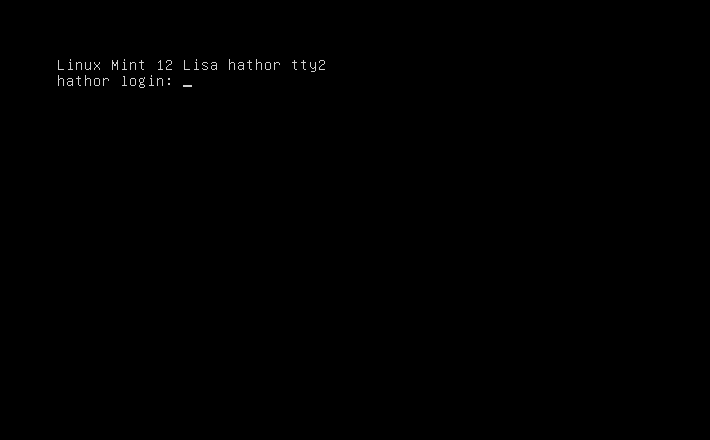
\includegraphics[width=0.7\linewidth,hight=0.7\linehight]{img/tty}
  \end{figure}
\end{frame}

\begin{frame}{Terminale (2)}
  \begin{itemize}
    \item pseudo-terminal
    \item gnome-terminal, konsole, xterm
  \end{itemize}
  \begin{figure}
    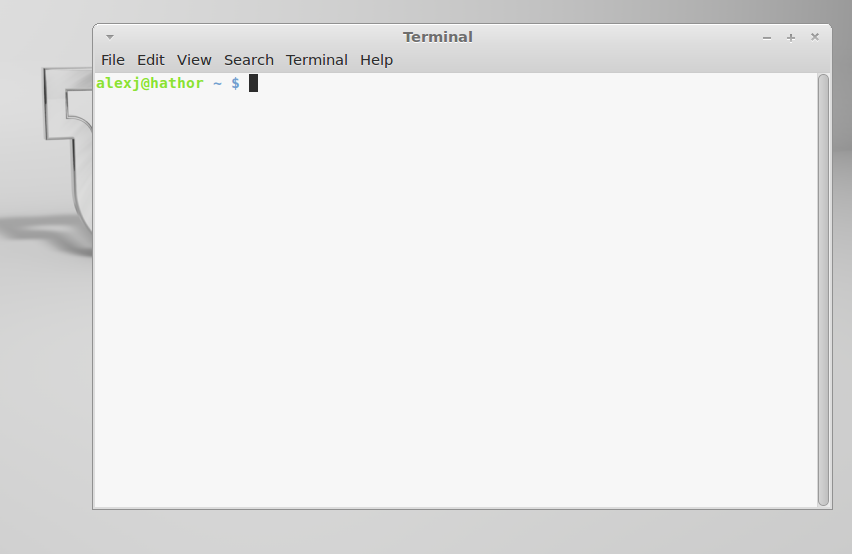
\includegraphics[width=0.7\linewidth,hight=0.7\linehight]{img/gnome-terminal}
  \end{figure}
\end{frame}

\begin{frame}{Terminale (3)}
  \begin{itemize}
    \item remote terminal
    \item ssh/telnet, putty
  \end{itemize}
  \begin{figure}
    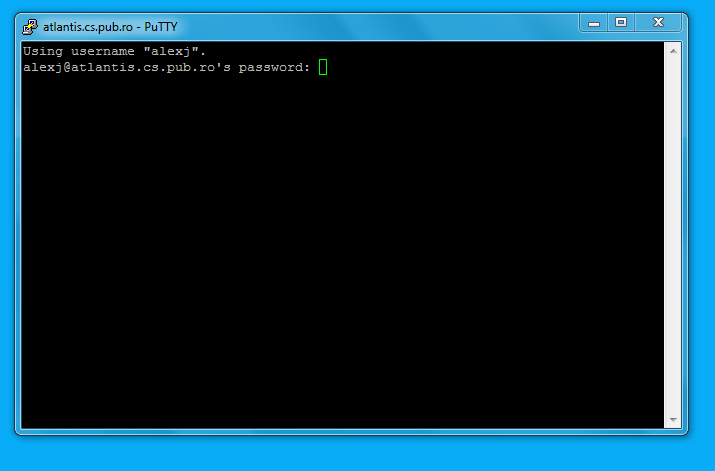
\includegraphics[width=0.7\linewidth,hight=0.7\linehight]{img/putty}
  \end{figure}
\end{frame}

\begin{frame}{Prompt}
  \begin{itemize}
    \item locul în care introducem comenzile
    \item conține informații utile: cine și unde suntem?
    \item diferă între CLI-uri
  \end{itemize}
  \begin{figure}
    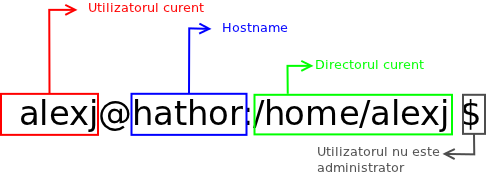
\includegraphics[width=0.7\linewidth,hight=0.7\linehight]{img/prompt}
  \end{figure}
\end{frame}

\begin{frame}{Structura unei comenzi}
  \begin{itemize}
    \item comenzi făra argumente
    \begin{itemize}
      \item \texttt{user@host\$ vim}
    \end{itemize}
    \item comenzi cu argumente
    \begin{itemize}
      \item argumentele se separă de comandă prin spațiu
      \item argumentele între ele se separă prin spațiu
      \item unele argumente pot fi flag-uri (precedate de - sau --)
      \item \texttt{user@host\$ ls -a}
      \item \texttt{user@host\$ ls --all}
      \item \texttt{user@host\$ ssh user@remotehost}
      \item \texttt{user@host\$ cp source.file destionation.file}
    \end{itemize}
  \end{itemize}
\end{frame}

\begin{frame}{Exemple de comenzi}
  \input{code/cli-example}
\end{frame}

\begin{frame}{Autocompletion}
  \begin{itemize}
    \item folosind tasta TAB
    \item se completează cel mai lung prefix neambiguu
    \item pentru afișarea sugestiilor se folosește TAB-TAB
  \end{itemize}
\end{frame}

\begin{frame}{Scurtături în shell}
  \begin{itemize}
    \item Ctrl-D -- logout
    \item Ctrl-C -- anulare comandă
    \item Alt-F/Alt-B -- deplasare cuvântul următor/anterior
    \item Ctrl-A/Ctrl-E -- deplasare începutul/sfârșitul liniei
    \item Alt-D -- șterge cuvântul curent
    \item Alt-Backspace -- șterge cuvântul anterior
  \end{itemize}
\end{frame}

\section{Folosirea sistemului Linux}

\begin{frame}{Clase de aplicații/comenzi}
  \begin{itemize}
    \item lucrul cu sistemul de fișiere
    \item lucrul cu procese
    \item instalarea de aplicații
    \item gestiunea utilizatorilor și drepturilor
    \item dezvoltarea de aplicații
    \item configurarea rețelei
    \item aplicații de rețea
    \item multimedia
    \item gestiunea documentelor
  \end{itemize}
\end{frame}

\begin{frame}{Lucrul cu sistemul de fișiere}
  \begin{itemize}
    \item fișier, director, link, separator
    \item poziționare și parcurgere: pwd, ls, cd
    \item crearea de fișiere: touch, mkdir, ln
    \item ștergerea de fișiere: rm, rm -r, rmdir
    \item afișarea fișierelor: cat, less, vi
    \item drepturi pe sisteme de fișiere: chmod, chown
  \end{itemize}
\end{frame}

\begin{frame}{Lucrul cu procese}
  \begin{itemize}
    \item procese, comunicarea între procese
    \item crearea de procese: \texttt{./executabil}
    \item listarea proceselor: ps, pstree, pgrep
    \item terminarea proceselor: kill, pkill
    \item monitorizarea proceselor: top, htop, lsof
  \end{itemize}
\end{frame}

\begin{frame}{Instalarea de aplicații}
  \begin{itemize}
    \item repository, pachet
    \item căutarea unui pachet: apt-cache search nume-pachet
    \item instalarea unui pachet: apt-get install nume-pachet
    \item ștergerea unui pachet: apt-get remove --purge nume-pachet
    \item inspectarea unui pachet: apt-cache show nume-pachet
    \item configurarea unui repository: /etc/apt/sources.list
    \item actualizarea bazei de date locale de pachete: apt-get update
    \item upgrade-ul sistemului: apt-get upgrade
  \end{itemize}
\end{frame}

\begin{frame}{Gestiunea utilizatorilor și drepturilor}
  \begin{itemize}
    \item utilizatori, grupuri, privilegii
    \item informații despre utilizatori: who, id, finger
    \item crearea unui utilizator: useradd
    \item ștergerea unui utilizator: userdel
    \item crearea unui grup: groupadd
    \item ștergerea unui grup: groupdel
    \item schimbarea parolei: passwd, chpasswd
    \item modificarea informațiilor: usermod
  \end{itemize}
\end{frame}

\begin{frame}{Dezvoltarea de aplicații}
  \begin{itemize}
    \item compilare, interpretare, biblioteci
    \item editarea codului sursă: Vim, Emacs, nano, Gedit, Kate, Jini
    \item compilarea/interpretarea surselor: gcc, g++, javac, python, php,
      perl, Make
    \item depanarea aplicațiilor: gdb, printf debugging
    \item rularea aplicațiilor: \texttt{./executabil}
    \item profiling: gprof, perf, oprofile
  \end{itemize}
\end{frame}

\begin{frame}{Configurarea rețelei}
  \begin{itemize}
    \item rețea, adresă, DNS
    \item vizualizarea informațiile de rețea: ifconig, route, arp, netstat, ip
    \item configurarea statică manuală: ifconfig, ip
    \item configurarea dinamică manuală: dhclient
    \item configurarea automată: /etc/network/interfaces
    \item configurarea server-ului de DNS: /etc/resolv.conf
    \item captură de pachete: tcpdump, wireshark, tshark
    \item depanare: route -n, ping, traceroute, host
  \end{itemize}
\end{frame}

\begin{frame}{Aplicații de rețea}
  \begin{itemize}
    \item web: server web, browsere, wget, curl, lynx
    \item email: server e-mail, server SMTP, Evolution, Thunderbird, mail,
      Mutt, Gnus
    \item SSH: server, ssh, scp, sftp
    \item DNS: sever, host, dig, nslookup
    \item BitTorrent: tracker, client
    \item monitorizare și captură: netstat, tcpdump, wireshark, lsof
  \end{itemize}
\end{frame}

\begin{frame}{Multimedia}
  \begin{itemize}
    \item viewere de imagini
    \item editoare de imagini: image-magick, Gimp
    \item viewere de filme
    \item convertoare de conținut de filme: ffmpeg, handbrake, kino
    \item playere de audio
    \item editoare de conținut audio: audacity
  \end{itemize}
\end{frame}

\begin{frame}{Gestiunea documentelor}
  \begin{itemize}
    \item editoare: Vim, Emacs, nano, Gedit, Kate
    \item suită Office: LibreOffice (OpenOffice), KOffice, Gnome Office
    \item LaTeX: latex, pdflatex, Kile, LyX
  \end{itemize}
\end{frame}

\section{Documentație}

\begin{frame}{Documentație în Linux}
  \begin{itemize}
    \item cel mai important skill: cum să înveți să găsești singur lucruri
    \item documentație disponibilă în sistem
    \begin{itemize}
       \item argumentele \texttt{-h} și \texttt{--help} la comenzi
       \item paginile de manual (comanda \texttt{man})
       \item paginile info (comanda \texttt{info})
       \item comenzi ajutătorare: \texttt{which}, \texttt{apropos}, \texttt{whatis}
    \end{itemize}
    \item documentație externă:
    \begin{itemize}
       \item The Linux Documentation Project (http://tldp.org)
       \item Google
       \item forumuri și liste de discuții
       \item IRC (live)
    \end{itemize}
  \end{itemize}
\end{frame}

\begin{frame}{Paginile de manual}
  \begin{itemize}
    \item man \texttt{comandă}
    \item căutare cu \texttt{/KEYWORD} și \texttt{n} și \texttt{N} pentru navigare
      \begin{itemize}
        \item \texttt{/KEYWORD} înseamnă ,,slash'' urmat de șirul de căutare
        \item \texttt{n} -- next
        \item \texttt{N} -- previous
        \item \texttt{?KEYWORD} pentru căutare înapoi
      \end{itemize}
    \item \emph{q} pentru ieșire
  \end{itemize}
\end{frame}

\section{Gestiunea pachetelor}

\begin{frame}{Distribuirea software-ului}
  \begin{itemize}
    \item tarballs (.tar, .tar.gz, .tgz)
    \begin{itemize}
      \item conțin surse, trebuiesc compilate
      \item necesită un toolchain pentru compilare
      \item sunt independente de platformă
      \item ``the Slackware way''
    \end{itemize}
    \pause
    \item package manager (.rpm, .deb)
    \begin{itemize}
      \item construite pentru o arhitectură/distribuție
      \item simplitate în administrare
      \begin{itemize}
        \item controlul versiunilor
        \item controlul dependențelor și al conflictelor
      \end{itemize}
    \end{itemize}
  \end{itemize}
\end{frame}

\begin{frame}{Debian Package Manager}
  \begin{itemize}
    \item folosit pe distribuții bazate pe Debian (inclusiv Ubuntu)
    \item pachet distribuit sub formă de fișier \texttt{.deb}
    \item \texttt{sendmail\_8.12.3-6.6.deb}
    \begin{itemize}
      \item sendmail -- numele pachetului
      \item 8.12.3 -- versiunea pachetului
      \item 6.6 -- versiunea distribuției pentru care este pachetul
    \end{itemize}
    \item utilitare
    \begin{itemize}
      \item dpkg
      \item apt-get
      \item apt-cache
      \item Synaptic, Aptitude
    \end{itemize}
  \end{itemize}
\end{frame}

\begin{frame}{APT (Advanced Packaging Tool)}
  \begin{itemize}
    \item caută și instalează pachete din locații specificate
    (\textbf{repositories})
    \item \texttt{/etc/apt/sources.list}
    \item \texttt{apt-get}
    \begin{itemize}
      \item update -- actualizează lista de pachete disponibile
      \item install -- instalează un pachet
      \item remove -- șterge un pachet
      \item uprade -- instalează o versiune mai nouă a unui pachet
    \end{itemize}
    \item mai nou \texttt{aptitude}
    \item \texttt{apt-cache}
    \begin{itemize}
      \item search -- caută un șir de caractere în numele și descrierile
      pachetelor din baza de date
    \end{itemize}
  \end{itemize}
\end{frame}

\begin{frame}{dpkg}
  \begin{itemize}
    \item back-end-ul folosit de \texttt{apt}
    \item folosit pentriu instalarea unor fișiere \texttt{.deb} (din afara
      repository-urilor)
    \item folosit pentru interogarea bazei de date locale cu pachete
      \begin{itemize}
        \item \texttt{dpkg -l '*alf*'} -- listează pachetele ce conțin șirul
          alf
        \item \texttt{dpkg -L procps} -- afișează fișierele din sistem care au
          fost instalate din cadrul pachetului \texttt{procps}
        \item \texttt{dpkg -S /usr/bin/which} -- din ce pachet face parte
          fișierul \texttt{/usr/bin/which}
      \end{itemize}
  \end{itemize}
\end{frame}

\section{Concluzie}

\begin{frame}{Cuvinte cheie}
  \begin{columns}
    \begin{column}[l]{0.5\textwidth}
      \begin{itemize}
        \item sistem de operare
        \item kernel
        \item Linux
        \item distribuții
        \item CLI
        \item shell
        \item terminal
        \item prompt
        \item comandă
        \item argumente
        \item autocompletion
      \end{itemize}
    \end{column}
    \begin{column}[l]{0.5\textwidth}
      \begin{itemize}
        \item operații în Linux
        \item man
        \item /KEYWORD
        \item apt-get
        \item /etc/apt/sources.list
        \item dpkg
      \end{itemize}
    \end{column}
  \end{columns}
\end{frame}

%\begin{frame}{Resurse utile}
%  \begin{itemize}
%    \item TODO
%  \end{itemize}
%\end{frame}

\section{Întrebări}

\end{document}
